\documentclass[11pt,a4paper]{article}
\usepackage[T1]{fontenc}
\usepackage[margin=2.3cm]{geometry}
\usepackage{amsmath,amssymb}
\usepackage{graphicx}
\usepackage[dvipsnames]{xcolor}
\usepackage{enumitem}
\usepackage[colorlinks=true,linkcolor=blue,urlcolor=blue]{hyperref}
\setlength{\parskip}{0.6em}
\setlength{\parindent}{0pt}
\begin{document}

\begin{center}{\LARGE\bfseries openprocesssim}\\[0.4em]{\large Build a small open process simulator: boxes, streams, a flash and a recycle loop, in three sessions.}\\[0.2em]\small PAN IIT OSS explainer \textbullet{} diploma / undergraduate to advanced undergraduate (levels 5-6)\end{center}

\section*{Why this exists}
Process simulators calculate how material and energy flow through a plant of connected units. This explainer shows how a learning-scale one works: streams, blocks, a flash, and the tear-stream trick that closes a recycle loop.

\section*{The end goal}
Build a small open process simulator with flash, heat exchanger and reactor blocks. The end goal is a small open process simulator with flash, heat exchanger and reactor blocks, in the spirit of commercial flowsheet tools but at learning scale. The ideas (graph, order, tear stream, degrees of freedom, closure) are the same as in industrial tools; this version uses ideal thermodynamics only and is not a design tool.

\section*{How the three sessions build up}
\begin{enumerate}[nosep]
\item \textbf{Session 1: Boxes, pipes and a loop: solve the rules together} (Level 1, conceptual interactive model, 60 min).
\item \textbf{Session 2: Streams, blocks and the flash: the numbers inside the boxes} (Level 2, mathematical engineering model, 80 min).
\item \textbf{Session 3: A flowsheet engine: graph, tear stream, closure and honest limits} (Level 3, simulation and validation, 90 min).
\end{enumerate}

\section{Session 1: Boxes, pipes and a loop: solve the rules together}

\subsection*{A. Real-world problem}
In a chemical plant a stream of liquid goes into a separator. The good part leaves as product and the rest is sent back to the start to try again. Every box obeys a simple rule (what goes in comes out), but because of the loop the flow into the first box depends on the flow out of the last. How much liquid really passes through the separator, and how does that change if we send more back? Flowsheet programs answer this for plants with hundreds of boxes; this repo builds a learning-scale analogue in the spirit of commercial flowsheet tools. Session 1 uses one number per pipe, a total flow in mol/s. It is a teaching model: real plants need process-safety engineering.

\subsection*{B. Concept and theory}
A flowsheet is a graph: boxes are the nodes and pipes (streams) are the lines between them. Name the streams: F = fresh feed (known), S = flow into the separator, P = product, R = recycle. Each box gives equations. The mixer joins F and R, so S = F + R. The separator sends a fraction r of S back and the rest out: R = r S and P = (1 - r) S. That is 3 unknowns (S, P, R) and 3 equations, so the plant can be solved. Written as a matrix, A x = b with x = [S, P, R], the computer solves all rules together in one step. The other way is to guess R, run the mixer and separator in order to get a new R, and repeat until the guess stops changing: successive substitution. For this loop the answer is S = F / (1 - r): at r = 0.5 the separator handles 2 times the feed, at r = 0.8 it handles 5 times and at r = 0.95 it handles 20 times.

\begin{itemize}[nosep]
\item F: fresh feed flow (known) (mol/s)
\item S: flow into the separator (mol/s)
\item P: product flow (mol/s)
\item R: recycle flow (mol/s)
\item r: recycle fraction, share of S sent back (0 to below 1) (no unit)
\end{itemize}

\begin{equation*}
S = F + R
\end{equation*}

\begin{equation*}
R = r\,S,\qquad P = (1-r)\,S
\end{equation*}

\begin{equation*}
\begin{pmatrix}1&0&-1\\-r&0&1\\-(1-r)&1&0\end{pmatrix}\begin{pmatrix}S\\P\\R\end{pmatrix}=\begin{pmatrix}F\\0\\0\end{pmatrix}\ \Rightarrow\ S=\frac{F}{1-r}
\end{equation*}

\begin{center}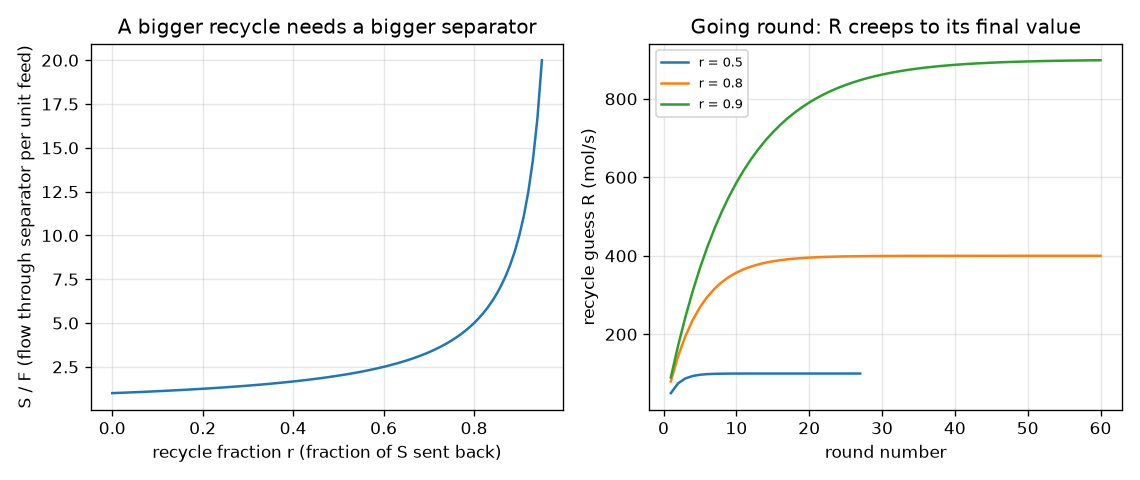
\includegraphics[width=0.85\linewidth]{figures/s01_loop.png}\\\small Left: separator flow per unit feed against the recycle fraction. Right: guess-and-go-round recycle guesses for r = 0.5, 0.8 and 0.9.\end{center}

\subsection*{E. Worked example}
A plant has a fresh feed F = 100 mol/s and a recycle fraction r = 0.6. Find S, R and P, and show the first three rounds of the guess-and-go-round method starting from R = 0.
\begin{enumerate}[nosep]
\item Mixer: S = F + R. Separator: R = 0.6 S and P = 0.4 S.
\item Substitute: S = 100 + 0.6 S, so 0.4 S = 100 and S = 250 mol/s.
\item Then R = 0.6 * 250 = 150 mol/s and P = 0.4 * 250 = 100 mol/s. Check: the product equals the fresh feed (100 = 100), as the overall balance demands.
\item Go round: guess R = 0, then S = 100 and the new R = 60. Next S = 160 and R = 96. Next S = 196 and R = 117.6. The guesses climb towards 150 and the code needs 37 rounds to get within 1e-6.
\end{enumerate}
\textbf{Answer.} S = 250 mol/s, R = 150 mol/s, P = 100 mol/s; the guesses go 60, 96, 117.6 and so on towards 150.

\subsection*{F. Questions}
\begin{enumerate}[nosep]
\item \textbf{Conceptual.} Why is the product flow equal to the fresh feed even though the separator handles much more?
\item \textbf{Numerical.} Find S, R and P for F = 100 mol/s and r = 0.75.
\item \textbf{Graph and simulation interpretation.} On the left figure, what does the separator handle per unit feed at r = 0.8 and at r = 0.95, and what does that mean for equipment size?
\item \textbf{Design and optimisation challenge.} Design: the separator can pass at most 400 mol/s. What is the largest recycle fraction at a feed of 100 mol/s, and what happens if the feed is raised to 150 mol/s? What would you trade away?
\end{enumerate}

\section{Session 2: Streams, blocks and the flash: the numbers inside the boxes}

\subsection*{A. Real-world problem}
A liquid mixture of benzene and toluene is heated until it just starts to boil, then a little more. Part of it turns into vapour, which is richer in the more volatile benzene. At what temperature does it start to boil, and how much vapour do we get at a chosen temperature? Inside a flowsheet program this question is answered thousands of times per solve; today you write that box. This is a teaching model with ideal liquids and gases and rounded textbook constants, not a design tool; benzene is also a hazardous chemical, and this repo only computes with it.

\subsection*{B. Concept and theory}
A stream carries the molar flow n\_i of each component (mol/s), a temperature T, a pressure P and a phase tag. With a constant liquid heat capacity Cp\_i, enthalpy relative to the pure liquids at 298.15 K is H = sum n\_i Cp\_i (T - 298.15), plus n\_i times the heat of vaporisation if the stream is vapour. The Antoine equation, log10(P\_sat / mmHg) = A - B / (C + T / degC), gives the vapour pressure of each pure liquid (rounded textbook constants for benzene, toluene and ethanol are in the lesson; 1 mmHg = 0.1333224 kPa). Raoult's law for an ideal mixture says the partial pressure of i is x\_i P\_sat\_i, so y\_i = K\_i x\_i with K\_i = P\_sat\_i / P. The bubble point is where sum x\_i P\_sat\_i = P, and the dew point is where sum y\_i / K\_i = 1; both are found by bisection on T. For a flash of a feed z at given T and P, the component balance z\_i = V y\_i + (1 - V) x\_i and the requirement that the vapour fractions add up to 1 give the Rachford-Rice equation f(V) = sum z\_i (K\_i - 1) / (1 + V (K\_i - 1)) = 0. f falls as V rises, so there is one root between 0 and 1, found by bisection or by Newton's method. For a given feed, a mixture boils over a window between its bubble and dew points; V is 0 at the bubble point and 1 at the dew point.

\begin{itemize}[nosep]
\item n\_i: molar flow of component i (mol/s)
\item z\_i, x\_i, y\_i: mole fraction in feed, liquid, vapour (no unit)
\item T, P: temperature and pressure (K, kPa)
\item P\_sat\_i: vapour pressure of pure i (kPa)
\item K\_i: K-value, y\_i / x\_i = P\_sat\_i / P (no unit)
\item V: vapour fraction, mol vapour per mol feed (no unit)
\item Cp\_i: liquid heat capacity (J/(mol K))
\item H: enthalpy flow (W)
\end{itemize}

\begin{equation*}
\log_{10}\frac{P^{sat}_i}{\mathrm{mmHg}}=A_i-\frac{B_i}{C_i+T/{}^\circ\mathrm{C}},\qquad K_i=\frac{P^{sat}_i}{P}
\end{equation*}

\begin{equation*}
\text{bubble: }\sum_i x_iP^{sat}_i(T)=P,\qquad \text{dew: }\sum_i \frac{y_i}{K_i}=1
\end{equation*}

\begin{equation*}
f(V)=\sum_i\frac{z_i(K_i-1)}{1+V(K_i-1)}=0,\qquad x_i=\frac{z_i}{1+V(K_i-1)},\quad y_i=K_ix_i
\end{equation*}

\begin{equation*}
H=\sum_i n_i\,Cp_i\,(T-298.15)\ \ (+\,n_i\Delta H^{vap}_i\text{ for vapour})
\end{equation*}

\begin{center}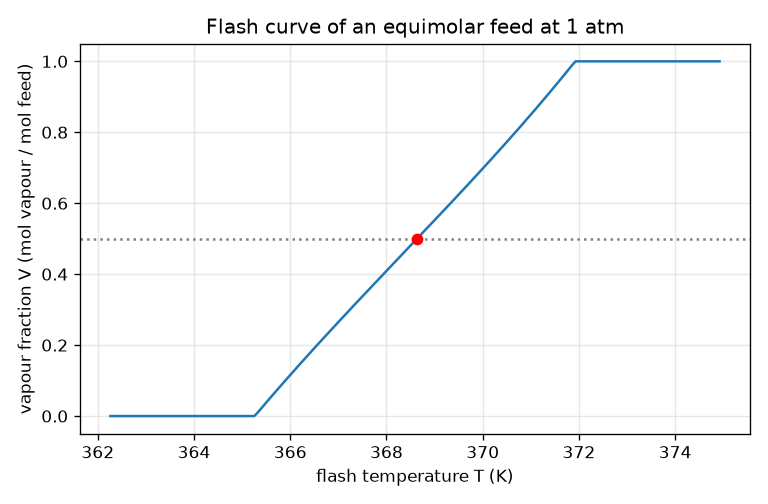
\includegraphics[width=0.85\linewidth]{figures/s02_flash_curve.png}\\\small Vapour fraction against flash temperature for the equimolar feed; the red dot is the 50 percent design point.\end{center}

\subsection*{E. Worked example}
An equimolar benzene-toluene feed (z = 0.5 each) at 1 atm (101.325 kPa) is flashed at 368 K. Find K-values, V, and the liquid and vapour compositions.
\begin{enumerate}[nosep]
\item Antoine at 368 K: P\_sat is 156.2 kPa for benzene and 63.3 kPa for toluene.
\item K = P\_sat / P: K\_benzene = 156.2 / 101.325 = 1.542 and K\_toluene = 63.3 / 101.325 = 0.6245.
\item Rachford-Rice: f(V) = 0.5 * 0.542 / (1 + 0.542 V) + 0.5 * (-0.3755) / (1 - 0.3755 V) = 0. Both ends of the interval are tested: f(0) is positive and f(1) is negative, so V is between 0 and 1. Bisection gives V = 0.409 (Newton's method needs 4 iterations, bisection 40 to reach 1e-12).
\item Liquid: x\_benzene = 0.5 / (1 + 0.409 * 0.542) = 0.409. Vapour: y\_benzene = 1.542 * 0.409 = 0.631.
\end{enumerate}
\textbf{Answer.} K = 1.542 and 0.6245, V = 0.409, liquid 0.409 benzene, vapour 0.631 benzene.

\subsection*{F. Questions}
\begin{enumerate}[nosep]
\item \textbf{Conceptual.} Why can a mixture not boil at a single temperature, as a pure liquid does?
\item \textbf{Numerical.} (a) How much heat does heating 100 mol/s of the equimolar liquid from 300 K to 350 K take? (b) What shaft power does a pump with 70 percent efficiency need to raise it by 400 kPa (molar volume 1e-4 m3/mol)? (c) What is the temperature after mixing 60 mol/s benzene at 300 K with 40 mol/s toluene at 340 K?
\item \textbf{Graph and simulation interpretation.} From the flash curve and T-x-y diagram: what is the highest benzene fraction any single flash of the equimolar feed can give in the vapour, and what temperature gives 50 percent vapour?
\item \textbf{Design and optimisation challenge.} Design: a flash of the equimolar feed at 1 atm must vaporise at least 30 percent of the feed and give a vapour with at least 0.65 benzene. Find the temperature window and say what a control engineer would worry about.
\end{enumerate}

\section{Session 3: A flowsheet engine: graph, tear stream, closure and honest limits}

\subsection*{A. Real-world problem}
A plant feeds mostly toluene. A reactor turns part of it into benzene, a flash separates a benzene-rich vapour, and the toluene-rich liquid is partly sent back to the start. A loop like that cannot be solved box by box in one pass, because the input of the first box depends on the output of the last. Commercial flowsheet tools solve this with a tear stream; here you build a small version of that engine. The reaction is a toy (toluene turning into benzene mole for mole, with no heat of reaction), the thermodynamics is ideal, and the result must never be used for plant design or safety decisions.

\subsection*{B. Concept and theory}
A flowsheet is a graph: blocks are nodes and streams are directed edges from the block that makes them to the block that uses them. If the graph has no loop, sort the blocks so that every block runs after the blocks that feed it (a topological order). If it has a loop, choose a tear stream: a stream whose removal leaves no loop. Guess the tear stream, run the blocks in order, and read the tear stream that comes back. Successive substitution uses what came back as the next guess. Wegstein acceleration estimates the slope s = (g\_k - g\_\{k-1\}) / (x\_k - x\_\{k-1\}) of the returned value g against the guess x and sets x\_next = q x + (1 - q) g with q = s / (s - 1), limited to -5 \textless{}= q \textless{}= 0. The blocks here are: mixer (adiabatic, outlet temperature from an energy balance), splitter (fraction r to the first outlet), conversion reactor (a fraction X of the toluene entering becomes benzene), heat exchanger (outlet temperature given, or UA with a utility at constant temperature T\_u, giving T\_out = T\_u - (T\_u - T\_in) exp(-UA / (n Cp)) and duty Q = n Cp (T\_out - T\_in)) and the isothermal flash of Session 2. Before solving, degrees of freedom are counted: DOF = settings given minus settings needed. DOF below 0 means under-specified, above 0 over-specified; the engine refuses both and says where. After solving, the engine reports mass closure (for each component, feed plus generation by reaction minus products out) and energy closure (enthalpy of products minus feeds minus the sum of block duties). A binary mixture in two phases at fixed T and P has no freedom left (phase rule), so the vapour and liquid compositions are fixed by T alone; recycle and conversion change the flows, not the purity. Raoult's law cannot represent an azeotrope: ethanol and benzene form a minimum-boiling azeotrope near 341 K at about 45 mole percent ethanol, whereas Raoult's law never gives a boiling point below the lowest pure boiling point.

\begin{itemize}[nosep]
\item F: fresh feed, 5 mol/s benzene + 95 mol/s toluene, 320 K (mol/s, K)
\item R: recycle (tear) stream (mol/s)
\item r: recycle fraction of the flash liquid (no unit)
\item X: conversion of toluene in the reactor (0.30) (no unit)
\item T\_flash: flash temperature (K)
\item UA: overall heat-transfer coefficient times area (W/K)
\item q: Wegstein acceleration factor (no unit)
\item DOF: degrees of freedom, settings given minus needed (count)
\end{itemize}

\begin{equation*}
x_{k+1}=g(x_k)\qquad(\text{successive substitution})
\end{equation*}

\begin{equation*}
x_{k+1}=q\,x_k+(1-q)\,g(x_k),\quad q=\frac{s}{s-1},\quad s=\frac{g(x_k)-g(x_{k-1})}{x_k-x_{k-1}},\quad -5\le q\le 0
\end{equation*}

\begin{equation*}
T_{out}=T_u-(T_u-T_{in})\,e^{-UA/(\dot n\,Cp)},\qquad Q=\dot n\,Cp\,(T_{out}-T_{in})
\end{equation*}

\begin{equation*}
\text{mass closure: }\sum_{\text{feeds}}n_i+\xi\,\nu_i-\sum_{\text{products}}n_i=0,\qquad \text{energy: }\sum H_{out}-\sum H_{in}=\sum Q
\end{equation*}

\begin{center}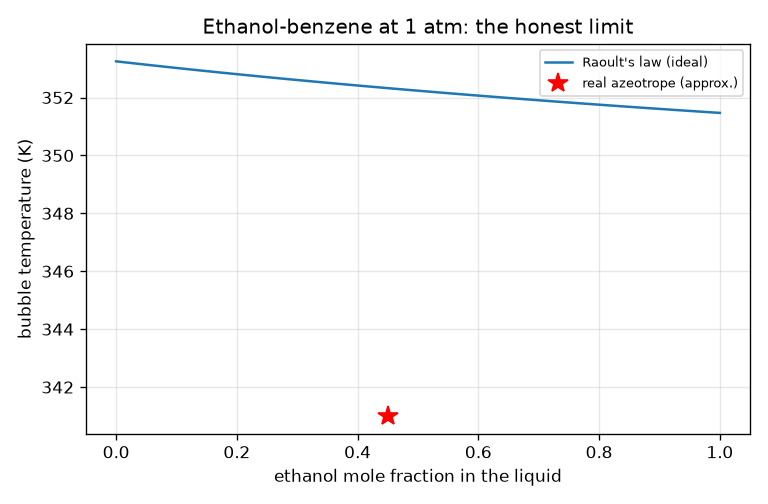
\includegraphics[width=0.85\linewidth]{figures/s03_azeotrope.png}\\\small Ethanol-benzene at 1 atm: Raoult's law against the approximate real azeotrope (red star).\end{center}

\subsection*{E. Worked example}
Solve the loop with the flash at only 345 K and r = 0.9, first by hand and then with the engine. Compare the iteration counts of substitution and Wegstein.
\begin{enumerate}[nosep]
\item Mixtures of benzene and toluene boil between 353.2 K and 383.8 K at 1 atm, so at 345 K nothing boils: V = 0 and the flash passes all its feed on as liquid.
\item The mixer and reactor conserve moles, so the flash feed is S = F + R = 100 + R and the liquid is L = S. The splitter returns R = 0.9 L.
\item So R = 0.9 (100 + R), 0.1 R = 90, R = 900 mol/s, and the bottoms are B = 0.1 * 1000 = 100 mol/s: the whole feed leaves as bottoms and nothing leaves as vapour product.
\item The engine agrees: R = 900 mol/s, B = 100 mol/s, V = 0. Substitution needs 263 iterations to reach 1e-10 (with a limit of 200 it stops short), Wegstein needs 34.
\end{enumerate}
\textbf{Answer.} R = 900 mol/s, B = 100 mol/s, V = 0; substitution 263 iterations, Wegstein 34. The loop converges but makes no vapour product, so the design is useless.

\subsection*{F. Questions}
\begin{enumerate}[nosep]
\item \textbf{Conceptual.} Why does a recycle loop need a tear stream?
\item \textbf{Numerical.} A heat exchanger heats 100 mol/s of toluene (Cp = 157 J/(mol K)) from 320 K with a utility at 400 K and UA = 15 700 W/K. Find T\_out and Q.
\item \textbf{Graph and simulation interpretation.} In the sensitivity figure, how do purity and product flow change between 364 and 372 K at r = 0.9, and does the recycle fraction move the purity curve?
\item \textbf{Design and optimisation challenge.} Design (the mini-project): find the highest flash temperature on a 0.5 K grid giving at least 0.70 benzene in the vapour, and the smallest r (0.05 grid) giving at least 60 mol/s of product. State the trade-off.
\end{enumerate}

\section{Real-world mini-project}
\textbf{Design a benzene recovery loop.} A feed of 100 mol/s (5 mol/s benzene, 95 mol/s toluene, liquid at 320 K) enters the loop of Session 3: mixer, reactor (30 percent of the toluene entering it turns into benzene, a toy reaction), heat exchanger, flash at 1 atm and a splitter that sends a fraction r of the flash liquid back. The shipped defaults (T = 368 K, r = 0.9) give a vapour product only 0.6311 benzene. Using \texttt{loop\_flowsheet}, \texttt{solve}, \texttt{closure} and \texttt{purity} from Session 3, find the highest flash temperature on a 0.5 K grid from 364 to 368 K for which the benzene purity of the vapour is at least 0.70, and then the smallest recycle fraction on a 0.05 grid from 0.5 to 0.95 for which the vapour product flow is at least 60 mol/s.

\section{The path ahead}
\begin{enumerate}[nosep]
\item \textbf{Session 4: Equation-oriented solving with Newton.} A Newton solver for the tear stream of the mini-project loop, with a damped step.
\item \textbf{Session 5: Non-ideal activity models.} Replace K = P\_sat / P with K = gamma P\_sat / P using a simple two-parameter model.
\item \textbf{Session 6: A rigorous distillation column.} A column block with N stages, reflux ratio and a feed stage.
\item \textbf{Session 7: A graphical flowsheet editor.} Save a flowsheet as JSON from a drawing, load it into the engine and solve it.
\item \textbf{Session 8: A property package.} A data file and loader, with water added as a fourth component.
\end{enumerate}

\section{Answers and hints}

\subsection*{Session 1}
\begin{enumerate}[nosep]
\item \textbf{Conceptual.} Hint: Draw a box around the whole plant and count only what crosses the box. Solution: At steady state nothing accumulates, so what enters the plant must leave it. Only the fresh feed crosses the plant boundary on the way in and only the product on the way out; the recycle stays inside. So P = F, however large S and R become.
\item \textbf{Numerical.} Hint: S = F / (1 - r), then R = r S and P = (1 - r) S. Solution: S = 100 / 0.25 = 400 mol/s, R = 0.75 * 400 = 300 mol/s, P = 0.25 * 400 = 100 mol/s. Units: mol/s throughout. Sanity check: P = F and S = F + R (400 = 100 + 300).
\item \textbf{Graph and simulation interpretation.} Hint: Read S / F off the curve. Solution: At r = 0.8 it handles 5 times the feed and at r = 0.95 it handles 20 times. Equipment is sized for S, not for F, so going from r = 0.8 to 0.95 makes the separator four times bigger for the same product.
\item \textbf{Design and optimisation challenge.} Hint: r = 1 - F / S\_max. Solution: r = 1 - 100 / 400 = 0.75 at 100 mol/s. At 150 mol/s the largest is r = 1 - 150 / 400 = 0.625 (check: S = 150 / 0.375 = 400). A lower recycle fraction means less of the 'not good enough' material gets a second chance, so in a real plant product quality or yield falls unless the separator is enlarged. This toy has no separation quality yet; Sessions 2 and 3 add it.
\end{enumerate}

\subsection*{Session 2}
\begin{enumerate}[nosep]
\item \textbf{Conceptual.} Hint: Compare the bubble and dew curves at the same composition. Solution: The more volatile component leaves first, so the liquid left behind becomes richer in the heavy component and its boiling temperature rises. The first vapour appears at the bubble point and the last liquid disappears at the dew point; between them both phases coexist. For the equimolar benzene-toluene mixture this window is 6.7 K wide.
\item \textbf{Numerical.} Hint: (a) Q = sum n Cp dT. (b) W = n v dP / eta. (c) Energy balance with the Cp values. Solution: (a) Cp mix = 0.5 * 136 + 0.5 * 157 = 146.5 J/(mol K), so Q = 100 * 146.5 * 50 = 732.5 kW. (b) W = 100 * 1e-4 * 400 000 / 0.7 = 5714 W = 5.71 kW. (c) T = 298.15 + (60 * 136 * 1.85 + 40 * 157 * 41.85) / (60 * 136 + 40 * 157) = 317.4 K. Units: W, W, K. Sanity checks: the mixed temperature lies between 300 and 340 K, and closer to 300 K because benzene is the larger flow.
\item \textbf{Graph and simulation interpretation.} Hint: The purest vapour is the very first vapour at the bubble point. Solution: The first vapour at the bubble point has 0.714 benzene and no flash of this feed can do better; as V grows the vapour gets leaner. 50 percent vapour needs 368.6 K, and then the vapour is 0.611 benzene and the liquid 0.389. A single flash cannot make a pure product, which is why columns and recycles exist.
\item \textbf{Design and optimisation challenge.} Hint: V \textgreater{}= 0.3 needs T \textgreater{}= 367.2 K. Purity falls as T rises; find where y drops below 0.65. Solution: 30 percent vapour needs 367.2 K, at which y = 0.655. The purity stays at or above 0.65 only up to 367.39 K (and is below 0.65 at 367.45 K). The window is only about 0.15 K wide, so the temperature controller must hold the flash to a fraction of a degree. In practice the target would be relaxed or a different pressure or an extra stage chosen. Assumptions: ideal mixture and approximate constants, so the true window will differ.
\end{enumerate}

\subsection*{Session 3}
\begin{enumerate}[nosep]
\item \textbf{Conceptual.} Hint: Try to find a run order of the blocks M, RX, HX, FL, SP without guessing anything. Solution: Every block needs its inputs before it can run, but in a loop each block waits for another (M needs R, which needs SP, which needs FL, ... which needs M). No order exists. Cutting the loop at one stream (the tear) and guessing it breaks the circle: the other blocks then have a valid order, and iteration makes the guess consistent with the result.
\item \textbf{Numerical.} Hint: n Cp = 15 700 W/K, so UA / (n Cp) = 1. Solution: T\_out = 400 - 80 * exp(-1) = 370.6 K. Q = 15 700 * (370.6 - 320) = 793.9 kW (equivalently the effectiveness 1 - exp(-1) = 0.632 times n Cp * 80 K). Units: K and W. Sanity check: T\_out lies between the inlet and the utility temperature.
\item \textbf{Graph and simulation interpretation.} Hint: Use the phase-rule remark in the theory. Solution: Purity falls from 0.7493 to 0.4973 while the product flow rises from 71.13 to 92.38 mol/s: a higher flash temperature vaporises more but dilutes the vapour. Changing r (0.5, 0.7 or 0.95) leaves the purity at 0.6311 (at 368 K) because in a binary two-phase flash the compositions are fixed by T and P; r only changes the flows (product 25.80, 83.70 and 98.33 mol/s at r = 0.5, 0.9, 0.99).
\item \textbf{Design and optimisation challenge.} Hint: At 365.5 K the purity is 0.7067 and at 366.0 K it is 0.6921; scan r at the chosen T. Solution: T = 365.5 K (366.0 K fails the purity target). At that T the product is 54.93 mol/s for r = 0.80 (fails) and 65.54 mol/s for r = 0.85 (passes), so r = 0.85. The recycle flow is then 195.25 mol/s and the bottoms 34.46 mol/s, with mass closure below 1e-8. The trade-off: a colder flash is purer but yields less vapour, and a larger recycle raises the product but makes every box and pipe in the loop handle more flow. Assumptions: ideal thermodynamics and a toy reaction.
\end{enumerate}

\section{How to join}
Read \texttt{CONTRIBUTING.md} in the repository, then pick an issue labelled \texttt{good first issue}. Repository: \url{https://github.com/KrunalPanchal1995/openprocesssim}

\end{document}
